%1. Plots of measured temp and peaks from interference.

%2. Results for thermal expansion coefficient, assume some distribution of heat.
% Prediction of material according to density, coefficient ...

%3. Error estimates for dt dL and L and coefficient
The experiment was conducted on two different metal rods that we denote as \emph{rod 1} and \emph{rod 2}.

\subsection{Results for Rod 1}
To determine the thermal expansion coefficients of rod 1, we analysed the normalized intensities measured by the photo diode. A sample of this data can be seen below in fig. \ref{fig:results:1}.

\begin{figure}[htb]
	\centering
	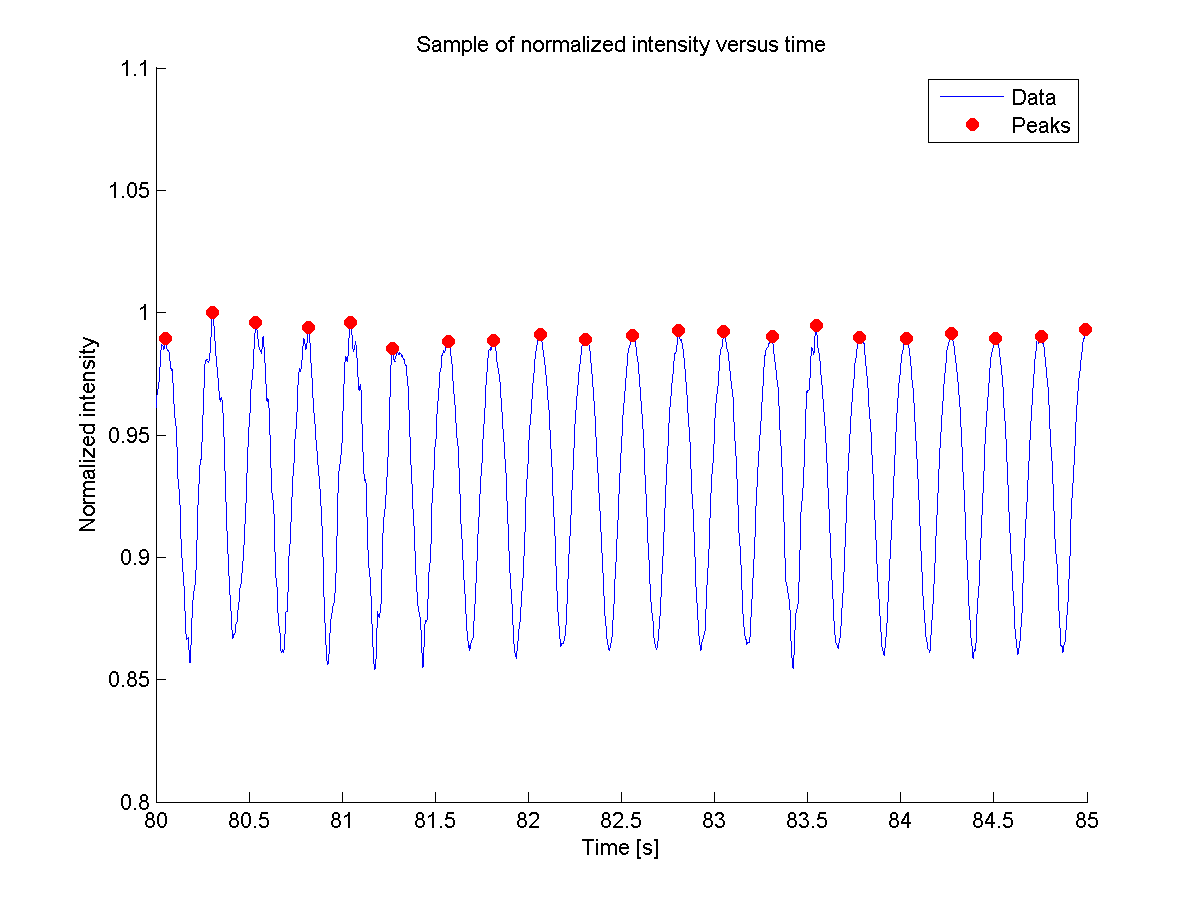
\includegraphics[width=0.8\textwidth]{img/Peaks_alu.png}
	\caption{A sample of the normalized intensity data measured by the photo diode. Peaks of the data is marked by circles.}
	\label{fig:results:1}
\end{figure}

\FloatBarrier
The peaks of the intensities were counted to calculate the linear expansion of the rod using eq. \eqref{eq7}.  
Temperature measurements were also analysed, raw data from the three temperature sensors can be seen below in fig. \ref{fig:results:2} and a calculated mean temperature in fig. \ref{fig:results:3}.
\begin{figure}[htb]
	\centering
	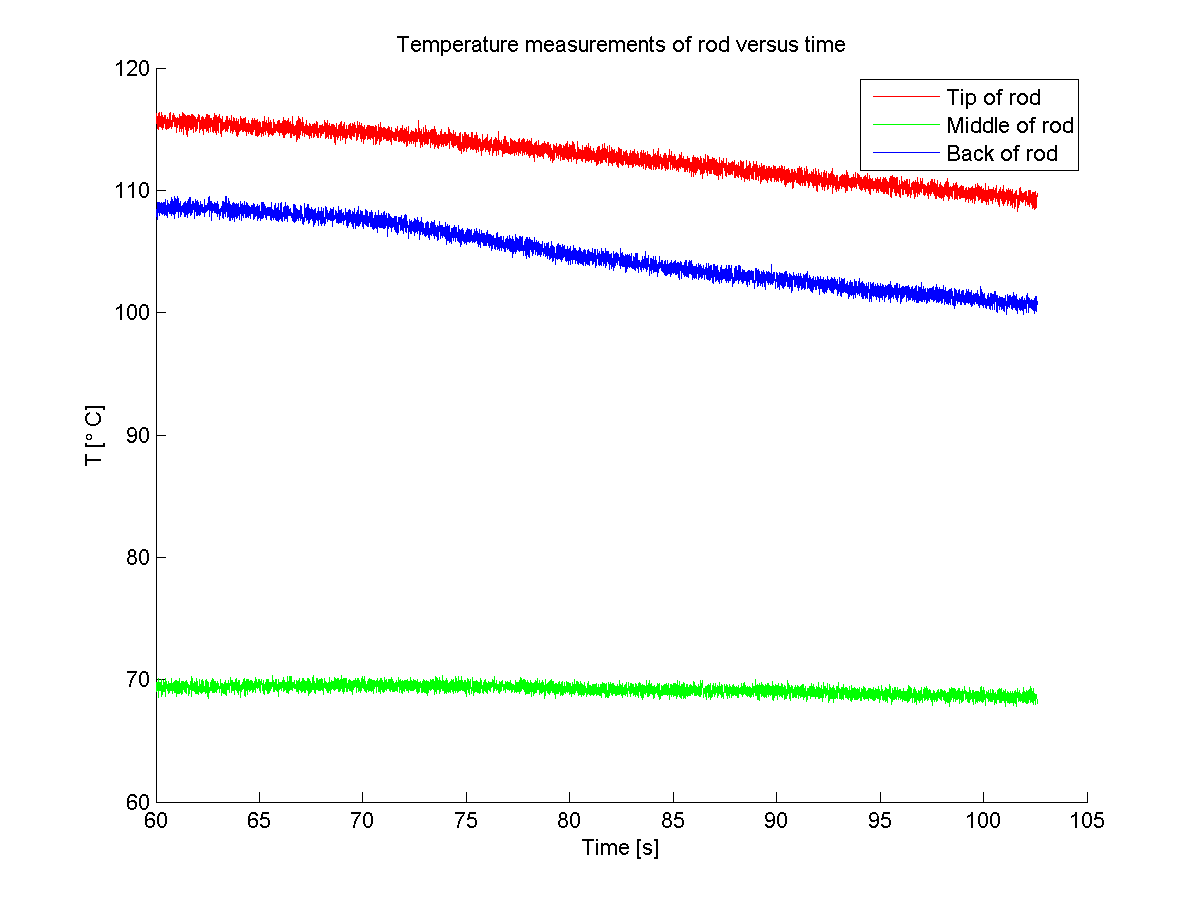
\includegraphics[width=0.8\textwidth]{img/temp_alu.png}
	\caption{Temperature measurements from the three thermistors mounted on the rod versus time.}
	\label{fig:results:2}
\end{figure}
\begin{figure}[htb]
	\centering
	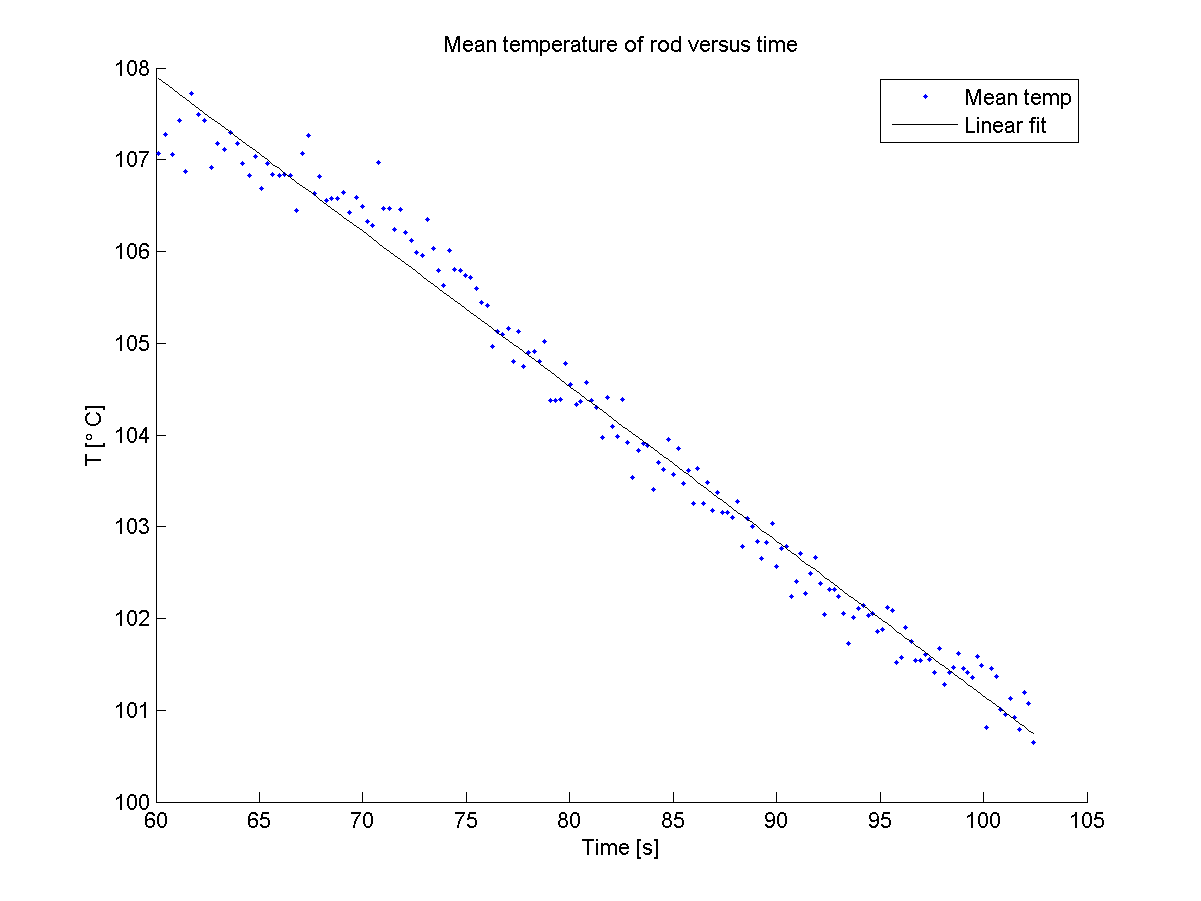
\includegraphics[width=0.8\textwidth]{img/mtemp_alu.png}
	\caption{Mean temperature of the rod versus time.}
	\label{fig:results:3}
\end{figure}
From this mean temperature the thermal expansion coefficient of Rod 1, $\alpha_1$, was calculated by using eq. \eqref{eq3}. The value obtained was 
$\alpha_1 =26.605 \cdot{10^{-6}} \; \rm{1/K}$.
The error estimate was calculated using \emph{Gauss propagation of uncertainty} and eq. \eqref{eq4} with
$L=0.280 \; \rm{m}$, $\Delta T = 7.1377 \; \rm{K}$ and $\Delta L = 5.3172 \cdot 10^{-6} \; \rm{m}$ with corresponding errors of $1 \; \rm{mm}$, $0.1 \; \rm{K}$ and $3.165 \cdot 10^{-7} \; \rm{m}$ respectively  to be $\sigma_{\alpha_1} = 0.416 \cdot 10^{-6} \; \rm{1/K}$.

A figure of the temperature dependency of the length expansion can be seen below in fig. \ref{fig:results:4}, assuming that this dependence is linear; eq. \eqref{eq4} is equal to eq. \eqref{eq3} and evaluations can be made for large $\Delta T$ and $ \Delta L$.

\begin{figure}[htb]
	\centering
	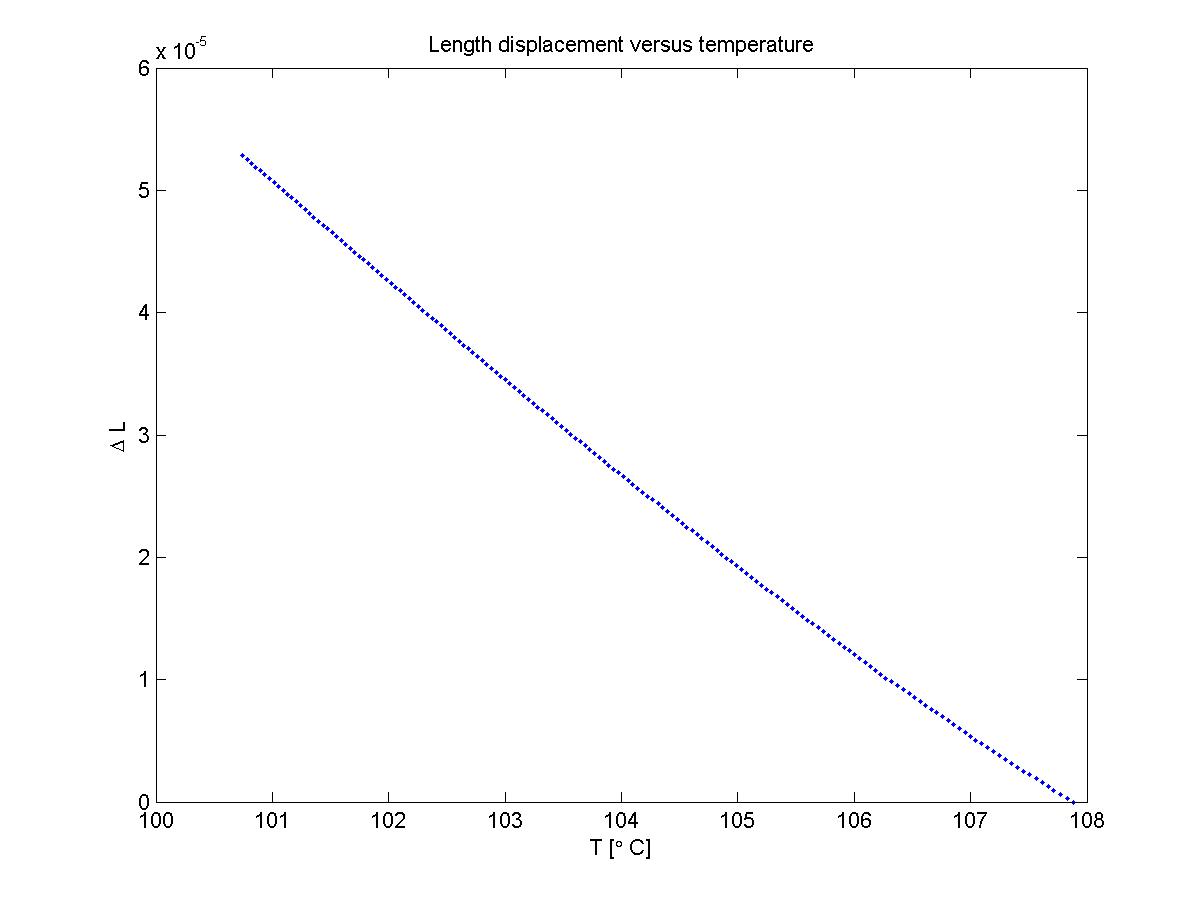
\includegraphics[width=0.8\textwidth]{img/dl_alu.png}
	\caption{Length expansion of the rod as a function of 		temperature.}
	\label{fig:results:4}
\end{figure}
\FloatBarrier

\subsection{Results for Rod 2}
The calculations described in the above sections where repeated for the second rod. Below we can find the corresponding figures, fig. \ref{fig:results:5},\ref{fig:results:6},\ref{fig:results:7} and \ref{fig:results:8} for these calculations.\\

\begin{figure}[htb]
	\centering
	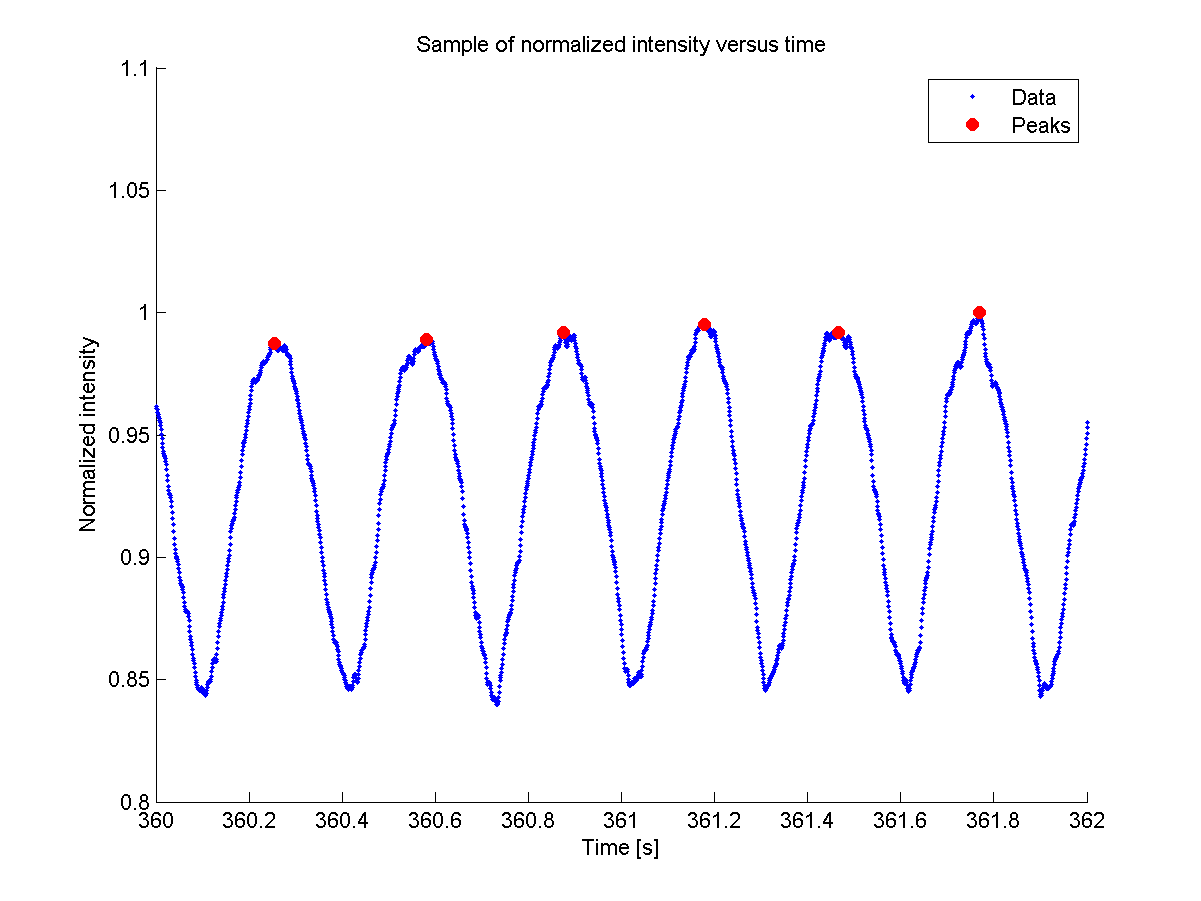
\includegraphics[width=0.8\textwidth]{img/Peaks_tit.png}
	\caption{A sample of the normalized intensity data measured by the photo diode. Peaks of the data is marked by circles.}
	\label{fig:results:5}
\end{figure}

\begin{figure}[htb]
	\centering
	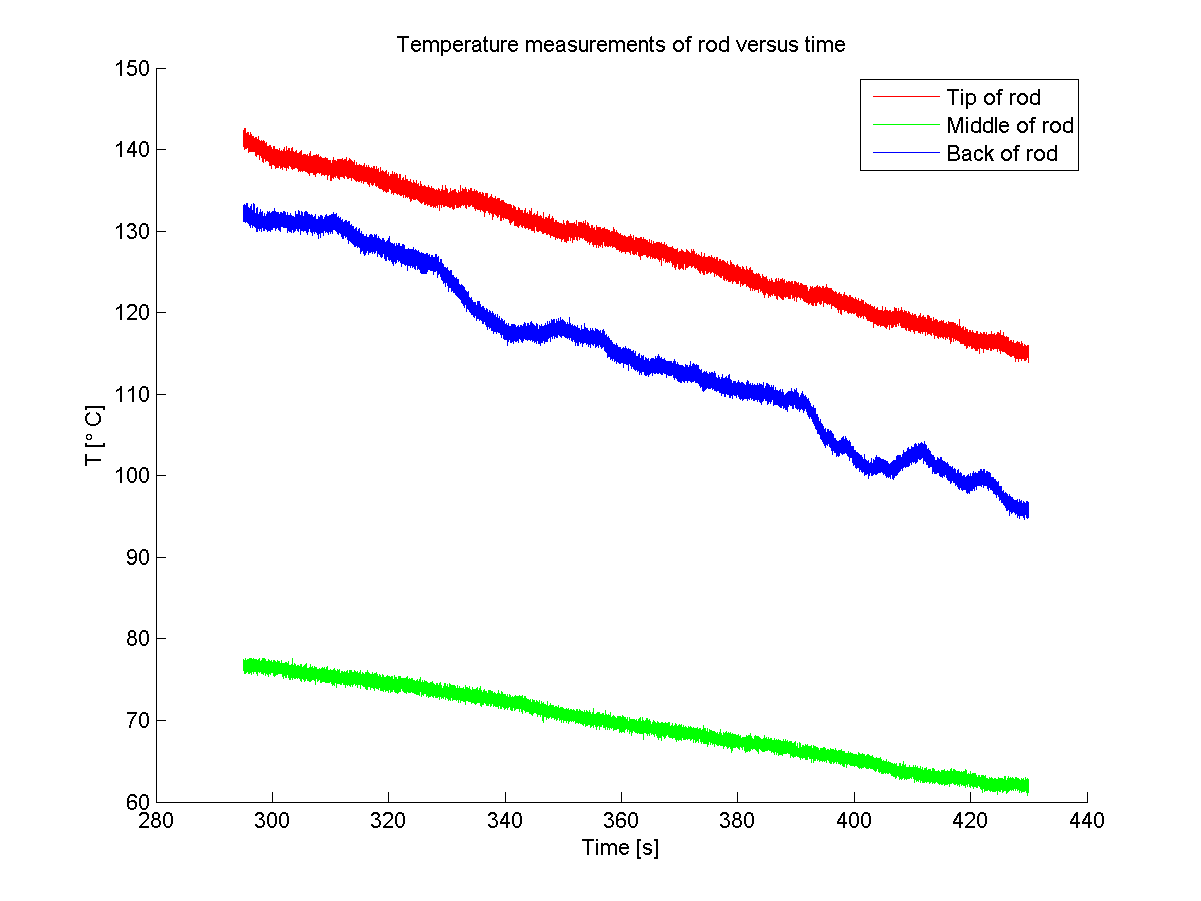
\includegraphics[width=0.8\textwidth]{img/temp_tit.png}
	\caption{Temperature measurements from the three thermistors mounted on the rod versus time.}
	\label{fig:results:6}
\end{figure}

\begin{figure}[htb]
	\centering
	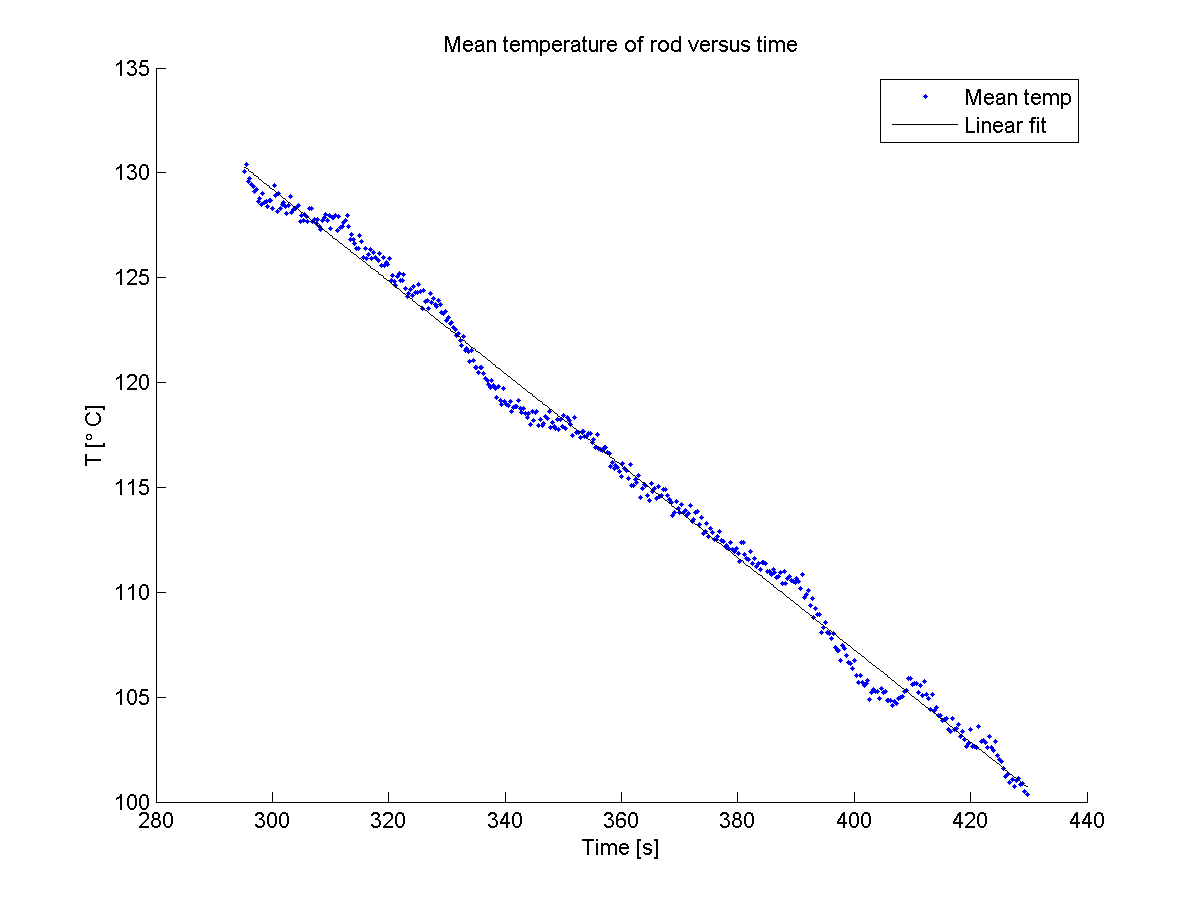
\includegraphics[width=0.8\textwidth]{img/mtemp_tit.png}
	\caption{Mean temperature of the rod versus time.}
	\label{fig:results:7}
\end{figure}

\begin{figure}[htb]
	\centering
	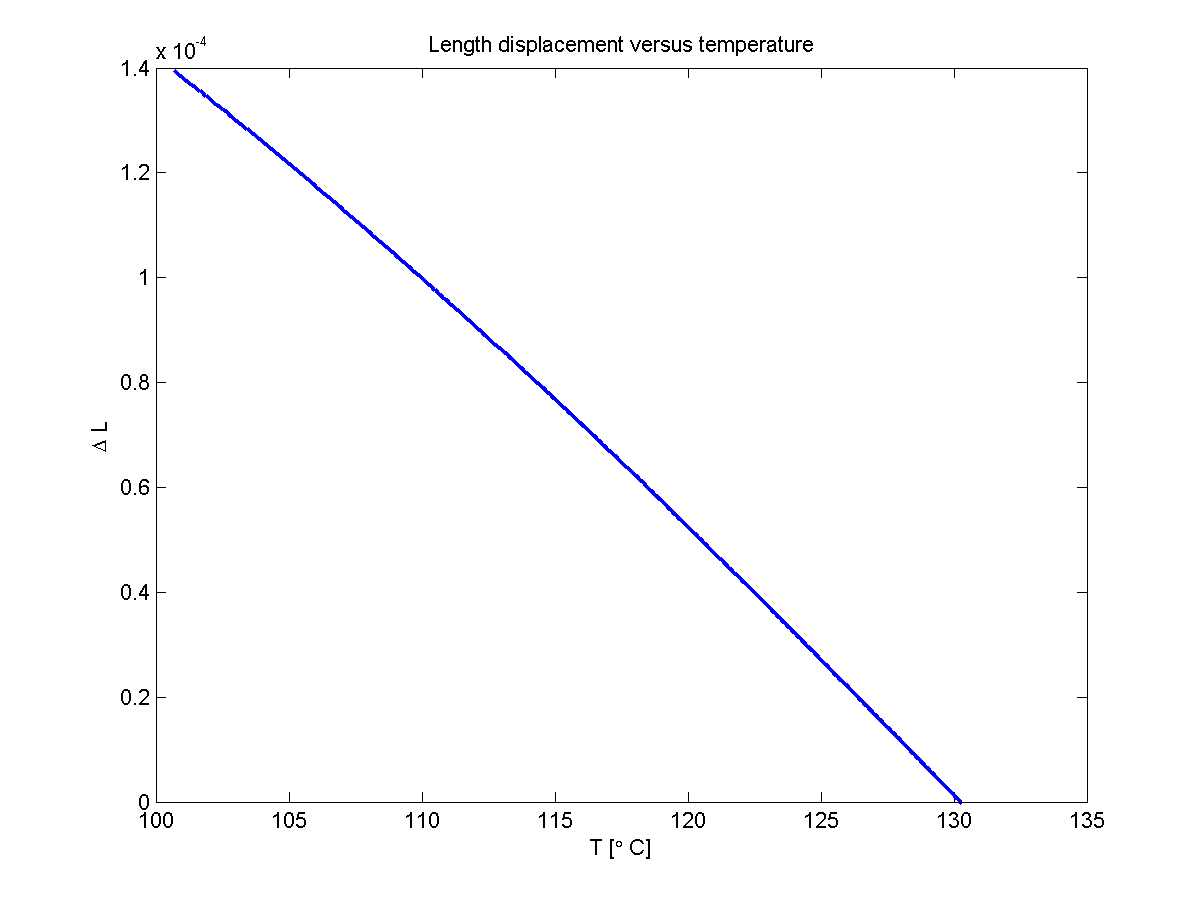
\includegraphics[width=0.8\textwidth]{img/dl_tit.png}
	\caption{Length expansion of the rod as a function of 		temperature.}
	\label{fig:results:8}
\end{figure}

\FloatBarrier
For this rod the thermal expansion coefficient was found to be $\alpha_2 = 19.371 \cdot 10^{-6}; 1/K$.
This error estimate was also calculated using \emph{Gauss propagation of uncertainty} and eq. \eqref{eq4}. But with
$L=0.245 \; \rm{m}$, $\Delta T = 30.6110 \; \rm{K}$ and $\Delta L =  1.4527 \cdot 10^{-4} \; \rm{m}$ with corresponding errors of $1 \; \rm{mm}$, $0.1 \; \rm{K}$ and $3.165 \cdot 10^{-7} \; \rm{m}$ respectively  to be $\sigma_{\alpha_2} =  0.110 \cdot 10^{-6} \; \rm{1/K}$.


